%%%%%%%%%%%%%%%%%%%%%%%%%%%%%%%%%%%%%%%%%%%%%%%%%%%%%%%%%%%%%%%
%% OXFORD THESIS TEMPLATE

% Use this template to produce a standard thesis that meets the Oxford University requirements for DPhil submission
%
% Originally by Keith A. Gillow (gillow@maths.ox.ac.uk), 1997
% Modified by Sam Evans (sam@samuelevansresearch.org), 2007
% Modified by John McManigle (john@oxfordechoes.com), 2015
% Modified by Ulrik Lyngs (ulrik.lyngs@cs.ox.ac.uk), 2018, for use with R Markdown
%
% Ulrik Lyngs, 25 Nov 2018: Following John McManigle, broad permissions are granted to use, modify, and distribute this software
% as specified in the MIT License included in this distribution's LICENSE file.
%
% John tried to comment this file extensively, so read through it to see how to use the various options.  Remember
% that in LaTeX, any line starting with a % is NOT executed.  Several places below, you have a choice of which line to use
% out of multiple options (eg draft vs final, for PDF vs for binding, etc.)  When you pick one, add a % to the beginning of
% the lines you don't want.


%%%%% CHOOSE PAGE LAYOUT
% The most common choices should be below.  You can also do other things, like replacing "a4paper" with "letterpaper", etc.

% This one will format for two-sided binding (ie left and right pages have mirror margins; blank pages inserted where needed):
%\documentclass[a4paper,twoside]{templates/ociamthesis}
% This one will format for one-sided binding (ie left margin > right margin; no extra blank pages):
%\documentclass[a4paper]{ociamthesis}
% This one will format for PDF output (ie equal margins, no extra blank pages):
%\documentclass[a4paper,nobind]{templates/ociamthesis}
%UL 2 Dec 2018: pass this in from YAML
\documentclass[a4paper, nobind]{templates/ociamthesis}

% UL 5 January 2021 - add packages used by kableExtra
\usepackage{booktabs}
\usepackage{longtable}
\usepackage{array}
\usepackage{multirow}
\usepackage{wrapfig}
\usepackage{colortbl}
\usepackage{pdflscape}
\usepackage{tabu}
\usepackage{threeparttable}
\usepackage{threeparttablex}
\usepackage[normalem]{ulem}
\usepackage{makecell}
\usepackage[colorlinks=false,pdfpagelabels,hidelinks=true]{hyperref}
\usepackage{float}

%UL set section header spacing
\usepackage{titlesec}
% 
\titlespacing\subsubsection{0pt}{24pt plus 4pt minus 2pt}{0pt plus 2pt minus 2pt}

% UL 30 Nov 2018 pandoc puts lists in 'tightlist' command when no space between bullet points in Rmd file
\providecommand{\tightlist}{%
  \setlength{\itemsep}{0pt}\setlength{\parskip}{0pt}}
 
% UL 1 Dec 2018, fix to include code in shaded environments
\usepackage{color}
\usepackage{fancyvrb}
\newcommand{\VerbBar}{|}
\newcommand{\VERB}{\Verb[commandchars=\\\{\}]}
\DefineVerbatimEnvironment{Highlighting}{Verbatim}{commandchars=\\\{\}}
% Add ',fontsize=\small' for more characters per line
\usepackage{framed}
\definecolor{shadecolor}{RGB}{248,248,248}
\newenvironment{Shaded}{\begin{snugshade}}{\end{snugshade}}
\newcommand{\AlertTok}[1]{\textcolor[rgb]{0.94,0.16,0.16}{#1}}
\newcommand{\AnnotationTok}[1]{\textcolor[rgb]{0.56,0.35,0.01}{\textbf{\textit{#1}}}}
\newcommand{\AttributeTok}[1]{\textcolor[rgb]{0.77,0.63,0.00}{#1}}
\newcommand{\BaseNTok}[1]{\textcolor[rgb]{0.00,0.00,0.81}{#1}}
\newcommand{\BuiltInTok}[1]{#1}
\newcommand{\CharTok}[1]{\textcolor[rgb]{0.31,0.60,0.02}{#1}}
\newcommand{\CommentTok}[1]{\textcolor[rgb]{0.56,0.35,0.01}{\textit{#1}}}
\newcommand{\CommentVarTok}[1]{\textcolor[rgb]{0.56,0.35,0.01}{\textbf{\textit{#1}}}}
\newcommand{\ConstantTok}[1]{\textcolor[rgb]{0.00,0.00,0.00}{#1}}
\newcommand{\ControlFlowTok}[1]{\textcolor[rgb]{0.13,0.29,0.53}{\textbf{#1}}}
\newcommand{\DataTypeTok}[1]{\textcolor[rgb]{0.13,0.29,0.53}{#1}}
\newcommand{\DecValTok}[1]{\textcolor[rgb]{0.00,0.00,0.81}{#1}}
\newcommand{\DocumentationTok}[1]{\textcolor[rgb]{0.56,0.35,0.01}{\textbf{\textit{#1}}}}
\newcommand{\ErrorTok}[1]{\textcolor[rgb]{0.64,0.00,0.00}{\textbf{#1}}}
\newcommand{\ExtensionTok}[1]{#1}
\newcommand{\FloatTok}[1]{\textcolor[rgb]{0.00,0.00,0.81}{#1}}
\newcommand{\FunctionTok}[1]{\textcolor[rgb]{0.00,0.00,0.00}{#1}}
\newcommand{\ImportTok}[1]{#1}
\newcommand{\InformationTok}[1]{\textcolor[rgb]{0.56,0.35,0.01}{\textbf{\textit{#1}}}}
\newcommand{\KeywordTok}[1]{\textcolor[rgb]{0.13,0.29,0.53}{\textbf{#1}}}
\newcommand{\NormalTok}[1]{#1}
\newcommand{\OperatorTok}[1]{\textcolor[rgb]{0.81,0.36,0.00}{\textbf{#1}}}
\newcommand{\OtherTok}[1]{\textcolor[rgb]{0.56,0.35,0.01}{#1}}
\newcommand{\PreprocessorTok}[1]{\textcolor[rgb]{0.56,0.35,0.01}{\textit{#1}}}
\newcommand{\RegionMarkerTok}[1]{#1}
\newcommand{\SpecialCharTok}[1]{\textcolor[rgb]{0.00,0.00,0.00}{#1}}
\newcommand{\SpecialStringTok}[1]{\textcolor[rgb]{0.31,0.60,0.02}{#1}}
\newcommand{\StringTok}[1]{\textcolor[rgb]{0.31,0.60,0.02}{#1}}
\newcommand{\VariableTok}[1]{\textcolor[rgb]{0.00,0.00,0.00}{#1}}
\newcommand{\VerbatimStringTok}[1]{\textcolor[rgb]{0.31,0.60,0.02}{#1}}
\newcommand{\WarningTok}[1]{\textcolor[rgb]{0.56,0.35,0.01}{\textbf{\textit{#1}}}}

%UL set white space before and after code blocks
\renewenvironment{Shaded}
{
  \vspace{10pt}%
  \begin{snugshade}%
}{%
  \end{snugshade}%
  \vspace{8pt}%
}

%UL set whitespace around verbatim environments
\usepackage{etoolbox}
\makeatletter
\preto{\@verbatim}{\topsep=0pt \partopsep=0pt }
\makeatother

%UL 26 Mar 2019, enable strikethrough
\usepackage[normalem]{ulem}

%UL use soul package for correction highlighting
\usepackage{color, soul}
\usepackage{xcolor}
\definecolor{correctioncolor}{HTML}{CCCCFF}
\sethlcolor{correctioncolor}
\newcommand{\ctext}[3][RGB]{%
  \begingroup
  \definecolor{hlcolor}{#1}{#2}\sethlcolor{hlcolor}%
  \hl{#3}%
  \endgroup
}
\soulregister\ref7
\soulregister\cite7
\soulregister\autocite7
\soulregister\textcite7
\soulregister\pageref7

%%%%%%% PAGE HEADERS AND FOOTERS %%%%%%%%%
\usepackage{fancyhdr}
\setlength{\headheight}{15pt}
\fancyhf{} % clear the header and footers
\pagestyle{fancy}
\renewcommand{\chaptermark}[1]{\markboth{\thechapter. #1}{\thechapter. #1}}
\renewcommand{\sectionmark}[1]{\markright{\thesection. #1}} 
\renewcommand{\headrulewidth}{0pt}

\fancyhead[LO]{\emph{\leftmark}} 
\fancyhead[RE]{\emph{\rightmark}} 

% UL page number position 
\fancyfoot[C]{\emph{\thepage}} %regular pages
\fancypagestyle{plain}{\fancyhf{}\fancyfoot[C]{\emph{\thepage}}} %chapter pages

% JEM fix header on cleared pages for openright
\def\cleardoublepage{\clearpage\if@twoside \ifodd\c@page\else
   \hbox{}
   \fancyfoot[C]{}
   \newpage
   \if@twocolumn\hbox{}\newpage
   \fi
   \fancyhead[LO]{\emph{\leftmark}} 
   \fancyhead[RE]{\emph{\rightmark}} 
   \fi\fi}


%%%%% SELECT YOUR DRAFT OPTIONS
% This adds a "DRAFT" footer to every normal page.  (The first page of each chapter is not a "normal" page.)

% This highlights (in blue) corrections marked with (for words) \mccorrect{blah} or (for whole
% paragraphs) \begin{mccorrection} . . . \end{mccorrection}.  This can be useful for sending a PDF of
% your corrected thesis to your examiners for review.  Turn it off, and the blue disappears.
\correctionstrue

%%%%% BIBLIOGRAPHY SETUP
% Note that your bibliography will require some tweaking depending on your department, preferred format, etc.
% If you've not used LaTeX before, I recommend reading a little about biblatex/biber and getting started with it.
% If you're already a LaTeX pro and are used to natbib or something, modify as necessary.
% Either way, you'll have to choose and configure an appropriate bibliography format...


\usepackage[style=authoryear, sorting=nyt, backend=biber, maxcitenames=2, useprefix, doi=true, isbn=false, uniquename=false]{biblatex}
\newcommand*{\bibtitle}{Works Cited}

\addbibresource{references.bib}


% This makes the bibliography left-aligned (not 'justified') and slightly smaller font.
\renewcommand*{\bibfont}{\raggedright\small}


% Uncomment this if you want equation numbers per section (2.3.12), instead of per chapter (2.18):
%\numberwithin{equation}{subsection}


%%%%% THESIS / TITLE PAGE INFORMATION
% Everybody needs to complete the following:
\title{Methods and applications of Bayesian spatio-temporal statistics for prioritised HIV prevention}
\author{Adam Howes}
\college{}

% Master's candidates who require the alternate title page (with candidate number and word count)
% must also un-comment and complete the following three lines:

% Uncomment the following line if your degree also includes exams (eg most masters):
%\renewcommand{\submittedtext}{Submitted in partial completion of the}
% Your full degree name.  (But remember that DPhils aren't "in" anything.  They're just DPhils.)
\degree{Doctor of Philosophy}
% Term and year of submission, or date if your board requires (eg most masters)
\degreedate{2023}


%%%%% YOUR OWN PERSONAL MACROS
% This is a good place to dump your own LaTeX macros as they come up.

\newcommand{\Sc}{\mathcal{S}}
\newcommand{\R}{\mathcal{R}}
\newcommand{\N}{\mathcal{N}}
\newcommand{\X}{\mathcal{X}} 
\newcommand{\m}{\mathbf{m}}
\newcommand{\bu}{\mathbf{u}}
\newcommand{\bv}{\mathbf{v}}
\newcommand{\w}{\mathbf{w}}
\newcommand{\x}{\mathbf{x}}
\newcommand{\y}{\mathbf{y}}
\newcommand{\z}{\mathbf{z}}
\newcommand{\bb}{\mathbf{b}}
\newcommand{\bphi}{\bm{\phi}}
\newcommand{\brho}{\bm{\rho}}
\newcommand{\btheta}{\bm{\theta}}

\RequirePackage{bm}

% To make text superscripts shortcuts
	\renewcommand{\th}{\textsuperscript{th}} % ex: I won 4\th place
	\newcommand{\nd}{\textsuperscript{nd}}
	\renewcommand{\st}{\textsuperscript{st}}
	\newcommand{\rd}{\textsuperscript{rd}}

%%%%% THE ACTUAL DOCUMENT STARTS HERE
\begin{document}

%%%%% CHOOSE YOUR LINE SPACING HERE
% This is the official option.  Use it for your submission copy and library copy:
\setlength{\textbaselineskip}{22pt plus2pt}
% This is closer spacing (about 1.5-spaced) that you might prefer for your personal copies:
%\setlength{\textbaselineskip}{18pt plus2pt minus1pt}

% You can set the spacing here for the roman-numbered pages (acknowledgements, table of contents, etc.)
\setlength{\frontmatterbaselineskip}{17pt plus1pt minus1pt}

% UL: You can set the line and paragraph spacing here for the separate abstract page to be handed in to Examination schools
\setlength{\abstractseparatelineskip}{13pt plus1pt minus1pt}
\setlength{\abstractseparateparskip}{0pt plus 1pt}

% UL: You can set the general paragraph spacing here - I've set it to 2pt (was 0) so
% it's less claustrophobic
\setlength{\parskip}{2pt plus 1pt}

%
% Oxford University logo on title page
%
\def\crest{{
\includegraphics{templates/ic-small.pdf}}}
\renewcommand{\university}{Imperial College London}
\renewcommand{\submittedtext}{A thesis submitted for the degree of}


% Leave this line alone; it gets things started for the real document.
\setlength{\baselineskip}{\textbaselineskip}


%%%%% CHOOSE YOUR SECTION NUMBERING DEPTH HERE
% You have two choices.  First, how far down are sections numbered?  (Below that, they're named but
% don't get numbers.)  Second, what level of section appears in the table of contents?  These don't have
% to match: you can have numbered sections that don't show up in the ToC, or unnumbered sections that
% do.  Throughout, 0 = chapter; 1 = section; 2 = subsection; 3 = subsubsection, 4 = paragraph...

% The level that gets a number:
\setcounter{secnumdepth}{2}
% The level that shows up in the ToC:
\setcounter{tocdepth}{1}


%%%%% ABSTRACT SEPARATE
% This is used to create the separate, one-page abstract that you are required to hand into the Exam
% Schools.  You can comment it out to generate a PDF for printing or whatnot.

% JEM: Pages are roman numbered from here, though page numbers are invisible until ToC.  This is in
% keeping with most typesetting conventions.
\begin{romanpages}

% Title page is created here
\maketitle

%%%%% DEDICATION -- If you'd like one, un-comment the following.
\begin{dedication}
  For \(\sum_i u_i\)
\end{dedication}

%%%%% ACKNOWLEDGEMENTS -- Nothing to do here except comment out if you don't want it.
\begin{acknowledgements}
 	Thanks to Jeff Eaton and Seth Flaxman for supervision of this research;
 staff and students of the StatML CDT at Imperial and Oxford;
 members of the HIV inference group at Imperial;
 Mike McLaren, Kevin Esvelt, the Nucleic Acid Observatory team, and the Sculpting Evolution lab for hosting my visit to MIT;
 Alex Stringer for hosting my visit to Waterloo;
 the Effective Altruism community;
 the Bill \& Melinda Gates Foundation and EPSRC for funding this PhD;
 my friends and family for their support.

 \begin{flushright}
 Adam Howes \\
 Imperial College London\\
 2023
 \end{flushright}
\end{acknowledgements}


%%%%% ABSTRACT -- Nothing to do here except comment out if you don't want it.
\begin{abstract}
	HIV remains a large problem.
Disease burden is unevenly distributed.
Effective public health response and prioritised prevention requires accurate, timely, high-resolution estimates of epidemic and demographic indicators.
Thoughtful statistical modelling is required to overcome significant data challenges.
In this thesis, I develop and apply Bayesian spatio-temporal methods for HIV surveillance.
\end{abstract}

%%%%% MINI TABLES
% This lays the groundwork for per-chapter, mini tables of contents.  Comment the following line
% (and remove \minitoc from the chapter files) if you don't want this.  Un-comment either of the
% next two lines if you want a per-chapter list of figures or tables.
  \dominitoc % include a mini table of contents

% This aligns the bottom of the text of each page.  It generally makes things look better.
\flushbottom

% This is where the whole-document ToC appears:
\tableofcontents

\listoffigures
	\mtcaddchapter
  	% \mtcaddchapter is needed when adding a non-chapter (but chapter-like) entity to avoid confusing minitoc

% Uncomment to generate a list of tables:
\listoftables
  \mtcaddchapter
%%%%% LIST OF ABBREVIATIONS
% This example includes a list of abbreviations.  Look at text/abbreviations.tex to see how that file is
% formatted.  The template can handle any kind of list though, so this might be a good place for a
% glossary, etc.
%tibble(
%  Term = c("HIV"),
%  Abbreviation = C("Human Immunodeficiency Virus")
%  ) %>%
%  arrange(Term) %>%
%  kable(booktab = TRUE, escape = FALSE, "latex")

% After writing, reorder these as they appear in the text

% First parameter can be changed eg to "Glossary" or something.
% Second parameter is the max length of bold terms.
\begin{mclistof}{List of Abbreviations}{3.2cm}

\item[HIV] Human Immunodeficiency Virus.
\item[DALY] Disability Adjusted Life Year.
\item[AIDS] Acquired ImmunoDeficiency Syndrome.
\item[UNAIDS] The Joint United Nations Programme on HIV/AIDS.
\item[PEPFAR] President’s Emergency Plan for AIDS Relief.
\item[Global Fund] Global Fund to Fight AIDS, Tuberculosis, and Malaria.
\item[HIV] Demographic and Health Surveys.
\item[AIS] AIDS Indicator Survey.
\item[PrEP] Pre-Exposure Prophylaxis.
\item[PEP] Post-Exposure Prophylaxis.
\item[FSW] Female Sex Worker(s).
\item[MSM] Men who have Sex with Men.
\item[PWID] People Who Inject Drugs.
\item[TGP] Transgender People
\item[ANC] Antenatal Clinic.
\item[CDC] Centers for Disease Control and Prevention.
\item[UAT] Unlinked Anonymous Testing.
\item[PMTCT] Prevention of Mother-to-Child Transmission.
\item[PLHIV] People Living with HIV.
\item[TaSP] Treatment as Prevention.
\item[STI] Sexually Transmitted Infection.
\item[ART] Antiretroviral Therapy.
\item[VMMC] Voluntary Medical Male Circumcision.
\item[DHS] Demographic and Health Surveys.
\item[PHIA] Population-based HIV Impact Assessment.
\item[SSA] Sub-Saharan Africa.

\item[DDC] Data Defect Correlation.
\item[MCMC] Markov Chain Monte Carlo.
\item[NUTS] No-U-Turn Sampler.
\item[VI] Variational Inference.
\item[INLA] Integrated Nested Laplace Approximation.
\item[GP] Gaussian Process.
\item[CAR] Conditionally Auto-regressive.
\item[ICAR] Intrinsic Conditionally Auto-regressive.
\item[SAE] Small-Area Estimation.
\item[GMRF] Gaussian Markov Random Field.
\item[HMC] Hamiltonian Monte Carlo.
\item[GMRF] Gauss-Markov Random Field.
\item[HMC] Hamiltonian Monte Carlo.
\item[LM] Linear Model.
\item[GLM] Generalised Linear Model.
\item[GLMM] Generalised Linear Mixed effects Model.
\item[LGM] Latent Gaussian Model.
\item[ELGM] Extended Latent Gaussian Model.
\item[BF] Bayes Factor.
\item[CPO] Conditional Predictive Ordinate.
\item[DIC] Deviance Information Criterion.
\item[BIC] Bayesian Information Criterion.
\item[WAIC] Watanabe-Akaike Information Criterion.
\item[SR] Scoring Rule.
\item[SPSR] Strictly Proper Scoring Rule.
\item[CRPS] Continuous Ranked Probability Score.
\item[LS] Log Score.
\item[PIT] Probability Integral Transform.
\item[ECDF] Empirical Cumulative Difference Function.
\item[ESS] Effective Sample Size.
\item[IID] Independent and Identically Distributed.
\item[PPL] Probabilistic Programming Language.
\item[CCD] Central Composite Design.
\item[EB] Empirical Bayes.
\item[AGHQ] Adaptive Gauss-Hermite Quadrature.

\end{mclistof} 


%%%%% LIST OF NOTATION
\begin{mclistof}{List of Notations}{3.2cm}

\item[$\rho$] HIV prevalence.
\item[$\lambda$] HIV incidence.
\item[$\alpha$] ART coverage.
\item[$\mathcal{S}$] Spatial study region $\mathcal{S} \subseteq \mathbb{R}^2$.
\item[$s \in \mathcal{S}$] Point location.
\item[$\mathcal{T}$] Temporal study period $\mathcal{T} \subseteq \mathbb{R}$.
\item[$t \in \mathcal{T}$] Time.
\item[$\y$] Data, a $n$-vector.
\item[$\bphi$] Parameters, a $d$-vector $(\phi_1, \ldots, \phi_d)$.
\item[$\x$] Latent field, a $N$-vector $(x_1, \ldots, x_N)$.
\item[$\btheta$] Hyperparameters, a $m$-vector $(\theta_1, \ldots, \theta_m)$.
\item[$x \sim p(x)$] $x$ is distributed according to $p(x)$.
\item[$A_i$] Areal unit.
\item[$A_i \sim A_j$] Adjacency between areal units.
\item[$\mathbf{H}$] Hessian matrix.
\item[$\mathbf{R}$] Structure matrix.
\item[$\mathbf{Q}$] Precision matrix.
\item[$\bm{\Sigma}$] Covariance matrix.
\item[$\mathcal{N}$] Gaussian distribution.
\item[$k: \mathcal{X} \times \mathcal{X} \to \mathbb{R}$] Kernel function on the space $\mathcal{X}$.
\item[$A_i \sim A_j$] Adjacency between areal units.
\item[$\mathcal{Q}$] A set of quadrature nodes.
\item[$\omega: \mathcal{Q} \to \mathbb{R}$] A quadrature weighting function.
\item[$\mathcal{Q}(m, k)$] Gauss-Hermite quadrature points in $m$ dimensions with $k$ nodes per dimension, constructed according to a product rule.

\end{mclistof} 

% The Roman pages, like the Roman Empire, must come to its inevitable close.
\end{romanpages}

%%%%% CHAPTERS
% Add or remove any chapters you'd like here, by file name (excluding '.tex'):
\flushbottom

% all your chapters and appendices will appear here
\hypertarget{background}{%
\chapter{Background}\label{background}}

\adjustmtc
\markboth{Background}{}

\hypertarget{small-area-estimation}{%
\section{Small-area estimation}\label{small-area-estimation}}

Small-area estimation methods aim to estimate population indicators for subgroups, typically in situations where direct estimates perform poorly due to data limitations.
These subgroups may often correspond to small geographic areas.
Small-area estimation methods have been used in a wide range of fields.
The Small-Area Health Statistics Unit (SASHU) at Imperial College London was set-up to monitor health around point sources of environmental pollution in response to the Sellafield enquiry into the increased incidence of childhood leukemia leukaemia near a nuclear reprocessing plant \autocite{elliott1992small}.
The research of SASHU has a focus on ratios of observed events to expected events, and testing hypothesis about hot-spots.

\hypertarget{the-hivaids-epidemic}{%
\section{The HIV/AIDS epidemic}\label{the-hivaids-epidemic}}

\begin{Shaded}
\begin{Highlighting}[]
\NormalTok{plhiv2022 }\OtherTok{\textless{}{-}} \DecValTok{38000000}
\NormalTok{deaths2022 }\OtherTok{\textless{}{-}} \DecValTok{700000}
\NormalTok{infections2022 }\OtherTok{\textless{}{-}} \DecValTok{1700000}
\end{Highlighting}
\end{Shaded}

According to latest estimates, in 2022 thirty-eight million people are living with HIV, there were seven hundred thousand AIDS-related deaths, and there were one million, seven hundred thousand people newly infected with HIV.
Surveillance is used is conducted to track epidemic trends, identify at-risk populations, find drivers of transmission, and evaluate the impact of prevention and treatment programs.
Sub-Saharan Africa is the most affected region.
Within sub-Saharan Africa, disease burden is unevenly distributed in space and across communities and individuals.
Key populations include men who have sex with men, female sex workers, people who inject drugs, transgender people, incarcerated people.
Larger demographic groups of higher risk include adolescent girls and young women.
Key HIV indicators are HIV prevalence, HIV incidence, coverage of ART and other interventions.
Key interventions are ART, condoms, PrEP and PEP, education, economic empowerment, VMMC.

There are significant data related difficulties associated with furnishing these estimates.
These include sparsity in space and time, survey bias, conflicting information sources, hard to reach populations, changing demographies.
These data limitations foreground the importance of synthesising multiple sources of information to obtain estimates.
Doing so increases the difficulty and complexity of the statistical modelling required.

Aims for HIV response going forward, and surveillance capabilities are needed to meet them.
Phasing out of nationally-representative household surveys for HIV.

Methods for prevention prioritisation include geographic, demographic, key population services, risk screening, individual-level risk characteristics.
Are there differences in effectiveness of treatments for different groups.

The population strategy \autocite{rose2001sick} is based on reducing risk factors across an entire population.
The individual strategy focuses on prevention in high-risk individuals.

\hypertarget{bayesian-spatio-temporal-statistics}{%
\section{Bayesian spatio-temporal statistics}\label{bayesian-spatio-temporal-statistics}}

Bayesian statistics is a statistical paradigm which, at its best, lets the analyst focus their attention on modelling the data at hand.
In particular, the primary concern is construction of a generative model for the observed data \(y\)
\[
(y, \vartheta) \sim p(y, \vartheta).
\]

Given a generative model, computation of the posterior distribution
\[
p(\vartheta \, | \, y) = \frac{p(y \, | \, \vartheta) p(\vartheta)}{p(y)}
\]
proceeds using approximate Bayesian inference methods.
Markov chain Monte Carlo (MCMC) is the most popular approach, and proceeds by simulating samples from a Markov chain with stationary distribution equal to the distribution of interest.
Variational Bayes approaches assume the posterior distribution belongs to some class and use optimisation to choose the best member of that class.
Particular properties of spatio-temporal models make integrated nested Laplace approximations, if feasible, often the best option
Empirical Bayes approaches, like Template Model Builder \autocite{osgoodzimmerman2021statistical}.

In spatio-temporal statistics the data we observe are indexed by spatial or temporal location.
The independent and identically distributed (IID) assumptions commonly used for observations are rarely suitable in this setting because we expect there to be spatio-temporal structure.
Split the parameters \(\vartheta = (x, \theta)\).
Call \(x\) the latent field.
Call \(\theta\) the hyperparameters.
Often, the latent field is assumed to be jointly multivariate Gaussian.

Latent Gaussian models \autocite{rue2009approximate} are of the form
\begin{align*}
y_i &\sim p(y_i \, | \, \eta_i, \theta_1), \quad i \in [n]\\
\mu_i &= \mathbb{E}(y_i \, | \, \eta_i) = g(\eta_i), \\
\eta_i &= \beta_0 + \sum_{l = 1}^{p} \beta_j z_{ji} + \sum_{k = 1}^{r} f_k(u_{ki}),
\end{align*}
where \([n] = \{1, \ldots, n\}\).
The response variable is \(y = (y)_{i \in [n]}\) with likelihood \(p(y \, | \, \eta, \theta_1) = \prod_{i = 1}^n p(y_i \, | \, \eta_i, \theta_1)\), where \(\eta = (\eta)_{i \in [n]}\).
Each response has conditional mean \(\mu_i\) with inverse link function \(g: \mathbb{R} \to \mathbb{R}\) such that \(\mu_i = g(\eta_i)\).
The vector \(\theta_1 \in \mathbb{R}^s\), with \(s_1\) assumed small, are additional parameters of the likelihood.
The structured additive predictor \(\eta_i\) may include an intercept \(\beta_0\), linear effects \(\beta_j\) of the covariates \(z_{ji}\), and unknown functions \(f_k(\cdot)\) of the covariates \(u_{ki}\).
The parameters \(\beta_0\), \(\{\beta_j\}\), \(\{f_k(\cdot)\}\) are each assigned Gaussian priors.
It is convenient to collect these parameters into a vector \(x \in \mathbb{R}^N\) called the latent field such that \(x \sim \mathcal{N}(0, Q(\theta_2)^{-1})\) where \(\theta_2 \in \mathbb{R}^{s_2}\) are further parameters, again with \(s_2\) assumed small.
Let \(\theta = (\theta_1, \theta_2) \in \mathbb{R}^s\) with \(m = s_1 + s_2\) be all hyperparameters, with prior \(p(\theta)\).
Common examples of latent Gaussian models include the following.

Many of the cutting-edge models used in small-area estimation fall outside the latent Gaussian model class.
Examples include disaggregation models, evidence synthesis models \autocite{eaton2019joint,eaton2021naomi}, attendance models, risk group models.
However, many of these models do fit into the class of extended latent Gaussian models \autocite{stringer2021fast}.
By allowing many-to-one link functions, extended latent Gaussian models facilitate modelling of non-linearities.

\hypertarget{understanding-models-for-spatial-structure}{%
\chapter{Understanding models for spatial structure}\label{understanding-models-for-spatial-structure}}

\adjustmtc
\markboth{Models for spatial structure}{}

Code for the analysis in this chapter is available from \href{https://github.com/athowes/areal-comparison}{\texttt{athowes/areal-comparison}} and supported by the R package \href{https://athowes.github.io/arealutils}{\texttt{arealutils}}.
Include an edited version of the corresponding paper here.

\hypertarget{background-1}{%
\section{Background}\label{background-1}}

\hypertarget{areal-and-point-data}{%
\subsection{Areal and point data}\label{areal-and-point-data}}

\hypertarget{spatial-random-effects}{%
\subsection{Spatial random effects}\label{spatial-random-effects}}

\hypertarget{models-based-on-adjacency}{%
\section{Models based on adjacency}\label{models-based-on-adjacency}}

\hypertarget{the-besag-model}{%
\subsection{The Besag model}\label{the-besag-model}}

\hypertarget{the-bym2-model}{%
\subsection{The BYM2 model}\label{the-bym2-model}}

\hypertarget{models-using-kernels}{%
\section{Models using kernels}\label{models-using-kernels}}

\hypertarget{the-centroid-kernel-model}{%
\subsection{The centroid kernel model}\label{the-centroid-kernel-model}}

\hypertarget{the-integrated-kernel-model}{%
\subsection{The integrated kernel model}\label{the-integrated-kernel-model}}

\hypertarget{simulation-study}{%
\section{Simulation study}\label{simulation-study}}

\hypertarget{synthetic-data-sets}{%
\subsection{Synthetic data-sets}\label{synthetic-data-sets}}

\hypertarget{inferential-models}{%
\subsection{Inferential models}\label{inferential-models}}

\hypertarget{priors}{%
\subsubsection{Priors}\label{priors}}

\hypertarget{kernel-details}{%
\subsubsection{Kernel details}\label{kernel-details}}

\hypertarget{inference-algorithms}{%
\subsection{Inference algorithms}\label{inference-algorithms}}

\hypertarget{model-assessment}{%
\subsection{Model assessment}\label{model-assessment}}

\hypertarget{continuous-ranked-probability-score}{%
\subsubsection{Continuous ranked probability score}\label{continuous-ranked-probability-score}}

\hypertarget{results}{%
\subsection{Results}\label{results}}

\hypertarget{hiv-prevalence-study}{%
\section{HIV prevalence study}\label{hiv-prevalence-study}}

\hypertarget{results-1}{%
\subsection{Results}\label{results-1}}

\hypertarget{discussion}{%
\section{Discussion}\label{discussion}}

\hypertarget{limitations}{%
\subsection{Limitations}\label{limitations}}

\hypertarget{conclusion}{%
\subsection{Conclusion}\label{conclusion}}

\hypertarget{multi-agyw}{%
\chapter{A multinomial spatio-temporal model for risk group proportions}\label{multi-agyw}}

\adjustmtc
\markboth{A multinomial spatio-temporal model for risk group proportions}{}

In this chapter I describe an application of Bayesian spatio-temporal statistics to small-area estimation of HIV risk group proportions.
This work was done in collaboration with colleagues from the MRC Centre for Global Infectious Disease Analysis and UNAIDS.
My role in the work was to develop the statistical model, building upon an earlier version of the analysis conducted by Kathryn Risher.
The results are described in \textcite{howes2023spatio}, and are now beginning to be used by countries to guide policy via a spreadsheet tool created by Kathryn.
Code for the analysis in this chapter is available from \href{https://github.com/athowes/multi-agyw}{\texttt{athowes/multi-agyw}} and supported by the R package \href{https://athowes.github.io/multi.utils}{\texttt{multi.utils}}.

\hypertarget{background-2}{%
\section{Background}\label{background-2}}

The risk of acquiring HIV infection is not equal for all individuals.

\hypertarget{data}{%
\section{Data}\label{data}}

I used the following household surveys.

\hypertarget{model-for-risk-group-proportions}{%
\section{Model for risk group proportions}\label{model-for-risk-group-proportions}}

I found that it was not appropriate to use the surveys without a specific transactional sex question on an equal footing as the other surveys.
For this reason, I took a two-stage modelling approach to estimating the four risk group proportions.
In particular, let the four risk groups be \(k \in \{1, 2, 3, 4\}\), and denote being in either the third or fourth risk group by \(k = 3^{+}\).
First, using all the surveys, I used a multinomial logistic regression model to model the proportion of AGYW in the risk groups \(k \in \{1, 2, 3^{+}\}\).
Then, using only those surveys with a specific transactional sex question, I fit a logistic regression model to estimate the proportion of those in the \(k = 3^{+}\) risk group that were in the \(k = 3\) and \(k = 4\) risk groups respectively.

\hypertarget{spatio-temporal-multinomial-logistic-regression}{%
\subsection{Spatio-temporal multinomial logistic regression}\label{spatio-temporal-multinomial-logistic-regression}}

\hypertarget{spatial-logistic-regression}{%
\subsection{Spatial logistic regression}\label{spatial-logistic-regression}}

\hypertarget{female-sex-worker-population-size-adjustment}{%
\subsection{Female sex worker population size adjustment}\label{female-sex-worker-population-size-adjustment}}

Responding ``yes'' to the survey question ``have you had sex in return for gifts, cash or anything else in the past 12 months'' is not considered sufficient to constitute sex work.
In recognition of this, I adjusted the estimates obtained based on the survey to match FSW population size estimates obtained via alternative methods.

\textcite{stevens2022estimating} used a Bayesian meta-analysis of key population specific data sources to estimate adult (15-49) FSW population size by country.
I disaggregated these estimates by age according to the following method.
First, I calculated the total sexually debuted population in each age group, in each country.
To describe the distribution of age at first sex, I used skew logistic distributions \autocite{nguyen2022trends} with cumulative distribution function given by
\begin{equation}
F(x) = \left(1 + \exp(\kappa_c (\mu_c - x)) \right)^{- \gamma_c},
\end{equation}
where \(\kappa_c, \mu_c, \gamma_c > 0\) are country-specific shape, shape and skewness parameters respectively.
Next, I used the assumed \(\text{Gamma}(\alpha = 10.4, \beta = 0.36)\) FSW age distribution in South Africa from the Thembisa model \autocite{johnson2020thembisa} to calculate the implied ratio between the number of FSW and the sexually debuted population in each age group.
I assumed these ratios in South Africa were applicable to every country, allowing calculation of the number of FSW by age group in all 13 countries.
The results obtained are shown in Figure \ref{fig:age-disagg-fsw-line}.

\begin{figure}
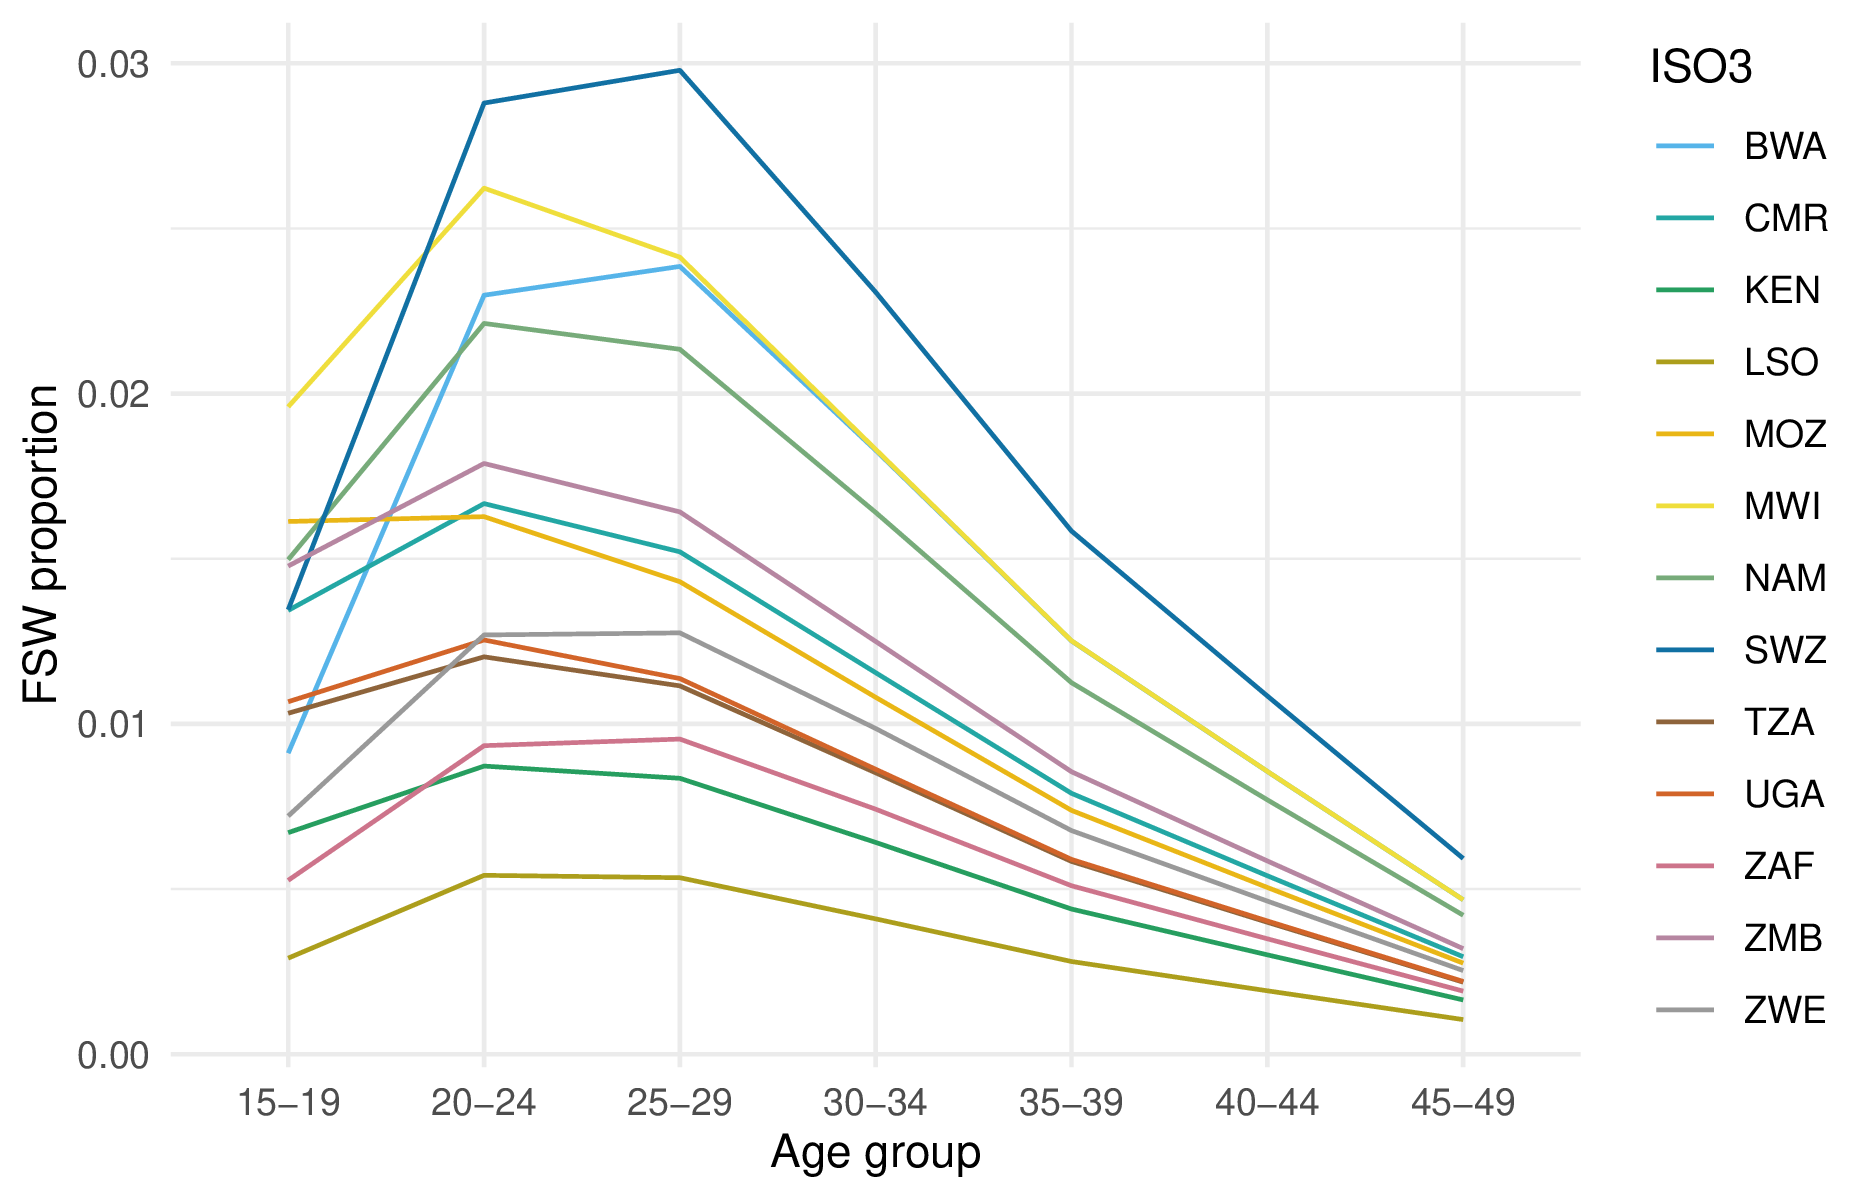
\includegraphics[width=0.9\linewidth]{figures/multi-agyw/age-disagg-fsw-line} \caption{Proportion of FSW by age group (including the age groups 30-34, 35-39, 40-44 and 45-49) as produced by the disaggregation procedure.}\label{fig:age-disagg-fsw-line}
\end{figure}

\hypertarget{results-2}{%
\subsection{Results}\label{results-2}}

\hypertarget{coverage-assessment}{%
\subsubsection{Coverage assessment}\label{coverage-assessment}}

\hypertarget{variance-decomposition}{%
\subsubsection{Variance decomposition}\label{variance-decomposition}}

\hypertarget{estimates}{%
\subsubsection{Estimates}\label{estimates}}

\hypertarget{calculation-of-prevalence-and-incidence-stratified-by-risk-group}{%
\section{Calculation of prevalence and incidence stratified by risk group}\label{calculation-of-prevalence-and-incidence-stratified-by-risk-group}}

\hypertarget{disaggregation-of-naomi-estimates}{%
\subsection{Disaggregation of Naomi estimates}\label{disaggregation-of-naomi-estimates}}

\hypertarget{expected-new-infections-reached}{%
\subsection{Expected new infections reached}\label{expected-new-infections-reached}}

\hypertarget{discussion-1}{%
\section{Discussion}\label{discussion-1}}

\hypertarget{limitations-1}{%
\subsection{Limitations}\label{limitations-1}}

\hypertarget{conclusion-1}{%
\subsection{Conclusion}\label{conclusion-1}}

\hypertarget{elgm-inf}{%
\chapter{Fast, approximate inference for the Naomi model}\label{elgm-inf}}

\adjustmtc
\markboth{Fast, approximate inference for the Naomi model}{}

Code for the analysis in this chapter is available from \href{https://github.com/athowes/elgm-inf}{\texttt{athowes/elgm-inf}} and supported by the R package \href{https://athowes.github.io/inf.utils}{\texttt{inf.utils}}.
Include an edited version of the corresponding paper here.

\hypertarget{future-work-and-conclusions}{%
\chapter{Future work and conclusions}\label{future-work-and-conclusions}}

\adjustmtc
\markboth{Conclusions}{}

\hypertarget{future-work}{%
\section{Future work}\label{future-work}}

Avenues for future work include:

\begin{enumerate}
\def\labelenumi{\arabic{enumi}.}
\tightlist
\item
  Extending the risk group model described in Chapter \ref{multi-agyw} to include all adults 15-49. This may involve modelling of age-stratified sexual partnerships \autocite{wolock2021evaluating}. Such a model would likely fall out of the scope of \texttt{R-INLA}, but may be possible using \texttt{aghq} with Laplace marginals as described in Chapter \ref{elgm-inf}.
\item
  Evaluating the accuracy of \texttt{aghq} with Laplace marginals for a greater variety of extended latent Gaussian models.
\end{enumerate}

\hypertarget{conclusions}{%
\section{Conclusions}\label{conclusions}}

The spatial structure chapter is interesting because:

\begin{itemize}
\tightlist
\item
  I designed experiments to thoroughly compare models for spatial structure using tools for model assessment such as proper scoring rules and posterior predictive checks.
\end{itemize}

The risk group chapter is interesting because:

\begin{itemize}
\tightlist
\item
  I estimated HIV risk group proportions for AGYW, enabling countries to prioritise their delivery of HIV prevention services.
\item
  I analysed the number of new infections that might be reached under a variety of risk stratification strategies.
\item
  I used \texttt{R-INLA} to specify multinomial spatio-temporal models via the Poisson-multinomial transformation. This includes complex two- and three-way Kronecker product interactions defined using the \texttt{group} and \texttt{replicate} options.
\end{itemize}

The fast, approximate inference chapter is interesting because:

\begin{itemize}
\tightlist
\item
  I developed a novel Bayesian inference method, motivated by a challenging and practically important problem in HIV inference.
\item
  The method enables integrated nested Laplace approximations to be fit to and studied on a wider class of models than was previously possible.
\item
  My implementation of the method was straightforward, building on the \texttt{TMB} and \texttt{aghq} packages, and described completely and accessibly in \textcite{howes2023integrated}.
\end{itemize}

My final conclusions are:

\begin{itemize}
\tightlist
\item
  Modelling complex data, more often than not, pushes the boundaries of the statistical toolkit available
\item
  A challenge I encountered was the difficulty of implementing identical models across multiple frameworks with the aim of studying the inference method. Or, of a similarly fraught nature, comparing different models implemented in different frameworks with the aim of studying model differences. The frequently asked questions section of the \texttt{R-INLA} website \autocite{rinla2023faq} notes that, ``the devil is in the details''. I have resolved this challenge by using a given \texttt{TMB} model template to fit models using multiple inference methodologies: empirical Bayes with Gaussian marginals \autocite{kristensen2016tmb}, AGHQ with Gaussian marginals \autocite{stringer2021implementing}, AGHQ with Laplace marginals \autocite{howes2023integrated}, and HMC using NUTS \autocite{monnahan2018no}. The benefits of such a ecosystem of packages are noted by \textcite{stringer2021fields}. I would particularly highlight the benefit of enabling analysts to easily vary their choice of inference method based on the stage of model development that they are in.
\item
  I have aimed to write this thesis, and the work described within it, in keeping with the principles of open science. I hope that doing so allows my work to be scrutinised, and, optimistically, built upon. This would not have been possible without a range of tools from the R ecosystem such as \texttt{rmarkdown} and \texttt{rticles}, as well as those developed within the MRC Centre for Global Infectious Disease Analysis like \texttt{orderly} and \texttt{didehpc}.
\end{itemize}

\startappendices

\hypertarget{the-first-appendix}{%
\chapter{The First Appendix}\label{the-first-appendix}}


%%%%% REFERENCES

% JEM: Quote for the top of references (just like a chapter quote if you're using them).  Comment to skip.
% \begin{savequote}[8cm]
% The first kind of intellectual and artistic personality belongs to the hedgehogs, the second to the foxes \dots
%   \qauthor{--- Sir Isaiah Berlin \cite{berlin_hedgehog_2013}}
% \end{savequote}

\setlength{\baselineskip}{0pt} % JEM: Single-space References

{\renewcommand*\MakeUppercase[1]{#1}%
\printbibliography[heading=bibintoc,title={\bibtitle}]}


\end{document}
